\begin{figure}
    \centering
    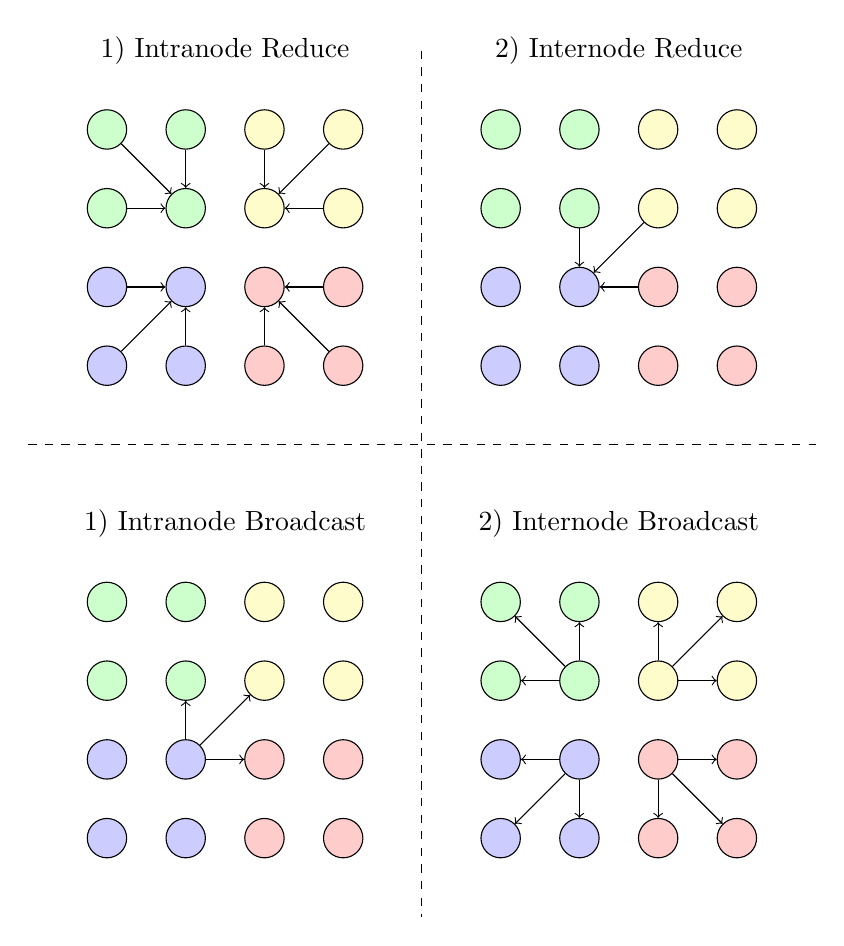
\begin{tikzpicture}[
        nsty/.style={
            draw,circle,
            minimum height=0.5cm,
        },
        csty0/.style={fill=blue!20},
        csty1/.style={fill=green!20},
        csty2/.style={fill=red!20},
        csty3/.style={fill=yellow!20},
    ]
    
    \foreach \n/\ox/\oy in {0/0/6,1/0/8,2/2/6,3/2/8}{
        \node[nsty,csty\n] at (\ox, \oy) (a0\n) {};
        \node[nsty,csty\n] at (1+\ox,\oy) (a1\n) {};
        \node[nsty,csty\n] at (\ox,1+\oy) (a2\n) {};
        \node[nsty,csty\n] at (1+\ox,1+\oy) (a3\n) {};
    }
    \draw[->] (a00) -- (a30);
    \draw[->] (a10) -- (a30);
    \draw[->] (a20) -- (a30);
    \draw[->] (a01) -- (a11);
    \draw[->] (a21) -- (a11);
    \draw[->] (a31) -- (a11);
    \draw[->] (a02) -- (a22);
    \draw[->] (a12) -- (a22);
    \draw[->] (a32) -- (a22);
    \draw[->] (a13) -- (a03);
    \draw[->] (a23) -- (a03);
    \draw[->] (a33) -- (a03);
    
    \foreach \n/\ox/\oy in {0/5/6,1/5/8,2/7/6,3/7/8}{
        \node[nsty,csty\n] at (\ox, \oy) (b0\n) {};
        \node[nsty,csty\n] at (1+\ox,\oy) (b1\n) {};
        \node[nsty,csty\n] at (\ox,1+\oy) (b2\n) {};
        \node[nsty,csty\n] at (1+\ox,1+\oy) (b3\n) {};
    }
    \draw[->] (b11) -- (b30);
    \draw[->] (b22) -- (b30);
    \draw[->] (b03) -- (b30);

    \foreach \n/\ox/\oy in {0/0/0,1/0/2,2/2/0,3/2/2}{
        \node[nsty,csty\n] at (\ox, \oy) (c0\n) {};
        \node[nsty,csty\n] at (1+\ox,\oy) (c1\n) {};
        \node[nsty,csty\n] at (\ox,1+\oy) (c2\n) {};
        \node[nsty,csty\n] at (1+\ox,1+\oy) (c3\n) {};
    }
    \draw[<-] (c11) -- (c30);
    \draw[<-] (c22) -- (c30);
    \draw[<-] (c03) -- (c30);

    
    \foreach \n/\ox/\oy in {0/5/0,1/5/2,2/7/0,3/7/2}{
        \node[nsty,csty\n] at (\ox, \oy) (d0\n) {};
        \node[nsty,csty\n] at (1+\ox,\oy) (d1\n) {};
        \node[nsty,csty\n] at (\ox,1+\oy) (d2\n) {};
        \node[nsty,csty\n] at (1+\ox,1+\oy) (d3\n) {};
    }
    \draw[<-] (d00) -- (d30);
    \draw[<-] (d10) -- (d30);
    \draw[<-] (d20) -- (d30);
    \draw[<-] (d01) -- (d11);
    \draw[<-] (d21) -- (d11);
    \draw[<-] (d31) -- (d11);
    \draw[<-] (d02) -- (d22);
    \draw[<-] (d12) -- (d22);
    \draw[<-] (d32) -- (d22);
    \draw[<-] (d13) -- (d03);
    \draw[<-] (d23) -- (d03);
    \draw[<-] (d33) -- (d03);

    \draw[dashed] (4,10) -- (4,-1);
    \draw[dashed] (-1,5) -- (9,5);
    \node[align=center] at (1.5, 10) {1) Intranode Reduce}; 
    \node[align=center] at (6.5, 10) {2) Internode Reduce}; 
    \node[align=center] at (1.5, 4) {1) Intranode Broadcast}; 
    \node[align=center] at (6.5, 4) {2) Internode Broadcast}; 
    
    \end{tikzpicture}
    \caption[Sixteen-Process Four-Node Hierarchical Allreduce]{
        A two-level hierarchical allreduce with 16 processes on 4 nodes, each colour representing a different node.
        The algorithm takes 4 steps, 1) intranode reduce, 2) internode reduce, 3) intranode broadcast, and 4) intranode broadcast.
    }
    \label{fig:sample_heir_allreduce}
\end{figure}